\section{Simulation Results}
\label{sec-simulations}

We have implemented the Firefly algorithm in TinyOS~\cite{tinyos-asplos00} using the 
TOSSIM~\cite{tossim} simulator environment. This simulator has several limitations. 
It does not model radio delay correctly, and nor does it take into account clock
skew that occurs from variations in clock crystals in individual wireless sensors. Despite these
limitations, the simulator is useful for exploring the parameter space of our 
algorithm.  This can help us determine optimal parameter settings for the algorithm on
a real testbed as well as better understand the impact of the parameter values on the 
level of synchronicity achieved.

In our simulator experiments, we explore the impact of varying: 

\begin{enumerate}\addtolength{\itemsep}{-0.5\baselineskip}
\item {\bf Node topology}: \emph{all-to-all} where each node can communicate with every other node, 
and a \emph{regular grid} topology where a node can directly exchange messages with at most
four other nodes.
\item {\bf Firing function constant value}: ranging from 10-1000. Recall from the theoretical
discussion of the algorithm that the time to synchronize is proportional to the firing
function constant value.
\item {\bf Number of nodes}: We examine whether the impact of the firing function constant and
node topology varies with the number of nodes. The size of the all-to-all topologies
is varied between 2-20 nodes with 2 node increments, and grid topologies are varied
from 16, 64, to 100 nodes.
\end{enumerate}

We evaluate these simulations using the two metrics defined in the previous section: {\bf Time to sync}
and {\bf 50th and 90th percentile group spread} and use them to determine the impact of the parameters
on the time taken to achieve synchronicity as well as the tightness of the synchronization.  

\subsection{Simulation Results}

Fig.~\ref{fig:alltts}-~\ref{fig:ata90} show the results of simulations on the all-to-all topology.
Each data point is averaged over several experimental runs. Although not shown here, error bars
for all the data points are also computed. Each experiment was run for 3600 seconds of 
simulation time with a unique random seed to start the nodes at different times.
We ran simulations for firing function constant values ranging from 10,20,50,70,100,150,300,500,750 and
1000, repeating this combination for number of nodes ranging from 2-20 with 2 node increments. 
Figure~\ref{fig:psynched} shows the percentage of cases that did not sync for these experiments.
Most experiments with firing function constant values of 10,2050 and 150 did not achieve
synchronicity. Consequently, we have suppressed the results for these experiments from the graphs
displaying the trends for the all-to-all topology.
%Table ~\ref{table:nosync} shows that this occurred particularly for a firing function constant value of 20.
%As explained in section 3.4, theoretical analysis predicts that the smaller the firing function
%constant value (i.e. large $\epsilon$), the larger a node jumps in response to other nodes,
%and thus nodes should converge to synchrony faster. 
One reason the simulation results for firing
function constant values in this range have this behavior this could be that the firing 
function constant value is too small, causing nodes to make extremely large jumps, and 
thus to miss firing at the times that their neighboring nodes are firing.

Fig.~\ref{fig:alltts} shows the time to sync for 2-20 nodes when the firing function 
constant is varied between 70-750.
Overall, the graph shows that the best (lowest) time to sync for different number
of nodes in an all-to-all topology can be achieved for firing constant values between 500-750.
While the time to sync does increase (for more than 2 motes) when the firing function constant value is varied from
500 to 750, the increase is less than 100 units of time and thus not significant.

\XXXnote{GT: This last para is crap. Needs to be rewritten.}
Fig.~\ref{fig:ata50} and Fig.~\ref{fig:ata90} show the extent of group spread 
in the 50th and 90th percentiles respectively for 2-20 nodes in an all-to-all 
topology. The graphs show that in most cases the tightness of the synchronicity decreases
with large values of the firing function constant.  The extent of this variation
in group spread, however is not very large. For instance the maximum change in the
group spread when the firing function constant values changes from 10 to 750 is
on the order of 2000 $\mu$seconds.

\begin{table}[t]
\begin{center}
\begin{tabular}{|c|c|c|} \hline
Topology & Number of Nodes & Firing Function Constant \\ \hline \hline
all-to-all &  2  &  1000 \\
all-to-all &  6  &  10 \\
all-to-all &  8  &  20 \\ 
all-to-all &  10 &  10 \\
all-to-all &  10 &  20 \\
all-to-all &  12 &  20 \\
all-to-all &  12 &  50 \\
all-to-all &  14 &  10 \\
all-to-all &  14 &  20 \\ 
all-to-all &  14 &  50 \\
all-to-all &  16 &  20 \\
all-to-all &  18 &  20 \\
all-to-all &  20 &  20 \\ 
grid       &  64 &  10 \\
grid       &  64 &  750 \\
grid       &  64 &  1000 \\
grid       &  100 &  750 \\
grid       &  100 &  1000 \\ \hline \hline
\end{tabular}
\end{center}
\caption{{\small Cases that did not achieve synchronicity consistently across all experimental runs.}}
\label{table:nosync}
\end{table}


\begin{figure}[p]
\begin{center}
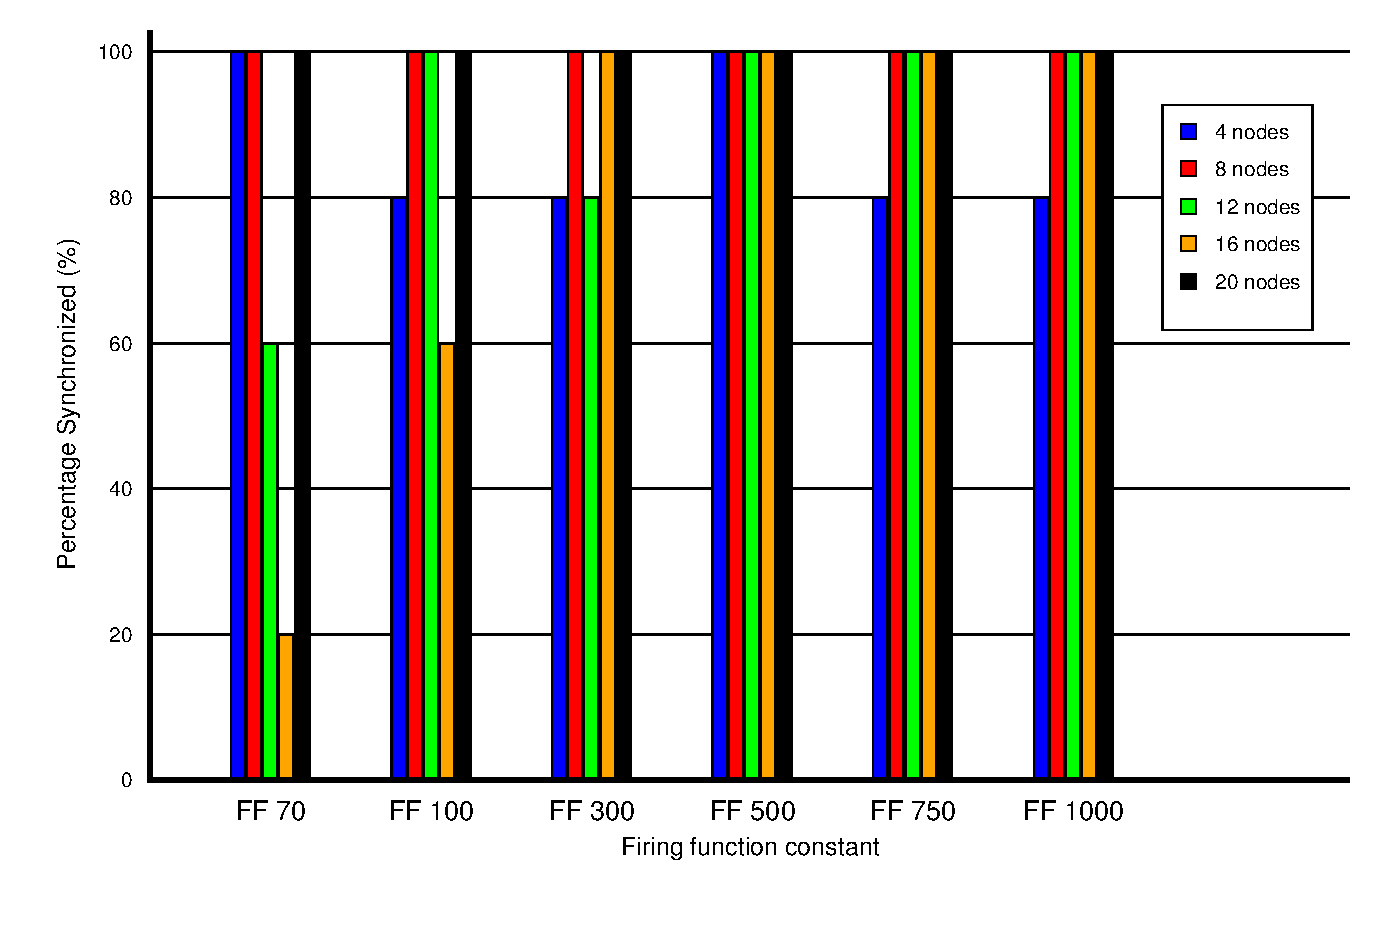
\includegraphics[width=1.0\hsize]{./figures/mdw/synch/percent-synch.pdf}
\end{center}
\caption{{\small {\bf Most experiments involving small firing function constants (E.g. 10,20,50,150) did not achieve synchronicity.}}}
\label{fig:alltts}
\end{figure}

\begin{figure}[p]
\begin{center}
\includegraphics[width=1.0\hsize]{./figures/mdw/ata/tts.pdf}
\end{center}
\caption{{\small {\bf Firing function constant values ranging between 500 and 750 produce the smallest time to synch for nodes in an all-to-all topology.}}}
\label{fig:alltts}
\end{figure}

\begin{figure}[p]
\begin{center}
\includegraphics[width=1.0\hsize]{./figures/mdw/ata/gs50.pdf}
\end{center}
\caption{{\small {\bf The tightness of synchronicity for half of the groups does not vary dramatically across different firing function constant values, but does increase with the number of nodes in an all-to-all topology.  The magnitude of the increase however is quite small.}}}
\label{fig:ata50}
\end{figure}

\begin{figure}[p]
\begin{center}
\includegraphics[width=1.0\hsize]{./figures/mdw/ata/gs90.pdf}
\end{center}
\caption{{\small {\bf 90th percentile group spread for different number of nodes in the all-to-all topology}}}
\label{fig:ata90}
\end{figure}

Fig.~\ref{fig:gridtts}-~\ref{fig:grid90} show the corresponding results for regular grid topologies.
Not suprisingly, the behavior of nodes in a grid topology changes dramatically from an all-to-all topology particularly
when the firing function constant is increased. In the grid topology, large values of the firing
function constant increase the time taken to achieve synchronicity and also decrease the tightness
of synchroncity. Nevertheless, Fig.~\ref{fig:grid90} shows that relatively tight synchronicity can be
achieved 90\% of the time even in the grid topology for any firing function constant value between 10 and 200.

\begin{figure}[p]
\begin{center}
\includegraphics[width=1.0\hsize]{./figures/mdw/grid/tts.pdf}
\end{center}
\caption{{\small {\bf The relationship between the firing function constant and the time to synch follows the theoretical predictions near-perfectly in a grid topology. In most cases the time to synch consistently increases as the firing function constant increases causing the nodes to make smaller jumps, thus converging to synchrony more slowly.}}}
\label{fig:gridtts}
\end{figure}

\begin{figure}[p]
\begin{center}
\includegraphics[width=1.0\hsize]{./figures/mdw/grid/gs50.pdf}
\end{center}
\caption{{\small {\bf The tightness of the synchronicity decreases with the number of nodes in the grid topology regardless of the number of nodes.  Furthermore, the firing function constant does not have a significant impact on the tightness of synchronicity in this topology.  These trends are retained in the 90th percentile group spread.}}}
\label{fig:grid90}
\end{figure}

\begin{figure}[p]
\begin{center}
\includegraphics[width=1.0\hsize]{./figures/mdw/grid/gs90.pdf}
\end{center}
\caption{{\small {\bf 90th percentile group spread in the grid topology for different number of nodes}}}
\label{fig:grid90}
\end{figure}


The simulation experiments proved beneficial in selecting parameter values for 
the experiments on the actual testbed of wireless sensors.  


